% Created 2020-07-07 mar 22:20
% Intended LaTeX compiler: pdflatex
\documentclass[presentation,aspectratio=1610]{beamer}
\usepackage[utf8]{inputenc}
\usepackage[T1]{fontenc}
\usepackage{graphicx}
\usepackage{grffile}
\usepackage{longtable}
\usepackage{wrapfig}
\usepackage{rotating}
\usepackage[normalem]{ulem}
\usepackage{amsmath}
\usepackage{textcomp}
\usepackage{amssymb}
\usepackage{capt-of}
\usepackage{hyperref}
\usepackage{khpreamble}
\usepackage{amssymb}
\DeclareMathOperator{\shift}{q}
\DeclareMathOperator{\diff}{p}
\usetheme{default}
\author{Kjartan Halvorsen}
\date{2020-07-08}
\title{Control Computarizado - Discretización de controladores continuos}
\hypersetup{
 pdfauthor={Kjartan Halvorsen},
 pdftitle={Control Computarizado - Discretización de controladores continuos},
 pdfkeywords={},
 pdfsubject={},
 pdfcreator={Emacs 26.3 (Org mode 9.3.6)}, 
 pdflang={English}}
\begin{document}

\maketitle


\section{Intro}
\label{sec:org8f7554b}

\section{Discretization}
\label{sec:org9f28dad}
\begin{frame}[label={sec:orgce53e41}]{Discretizing a controller}
\begin{itemize}
\item Have a controller \(F(s)\) obtained from a design in continuous time.
\item Discretize in order to implement on a computer
\end{itemize}

\begin{center}
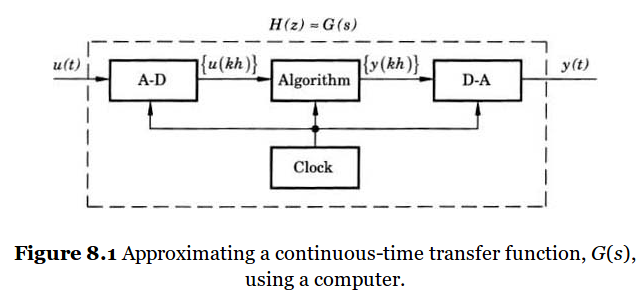
\includegraphics[width=0.7\linewidth]{../../figures/fig8-1.png}
\end{center}
\end{frame}

\begin{frame}[label={sec:org51419b3}]{Discretization methods}
\begin{enumerate}
\item Forward difference. Substitute 
\[ s = \frac{z-1}{h} \] in \(F(s)\) to get
\[ F_d(z) = F(s')|_{s'=\frac{z-1}{h}}. \]
\item Backward difference. Substitute 
\[ s = \frac{z-1}{zh} \] in \(F(s)\) to get
\[ F_d(z) = F(s')|_{s'=\frac{z-1}{zh}}. \]
\end{enumerate}
\end{frame}
\begin{frame}[label={sec:org44a4d27}]{Discretization methods, contd.}
\begin{enumerate}
\setcounter{enumi}{2}
\item Tustin's method (also known as the bilinear transform). Substitute
\[ s = \frac{2}{h}\frac{z-1}{z+1} \] in \(F(s)\) to get
\[ F_d(z) = F(s')|_{s'=\frac{2}{h}\cdot \frac{z-1}{z+1}}. \]
\item Ramp invariance. This is similar to ZoH, which is step-invariant approximation. 
Since a unit ramp has z-transform \(\frac{zh}{(z-1)^2}\) and Laplace-transform \(1/s^2\),  the discretization becomes
\[ F_d(z) = \frac{(z-1)^2}{zh} \ztrf{\laplaceinv{\frac{F(s)}{s^2}}}. \]
\end{enumerate}
\end{frame}

\begin{frame}[label={sec:org7cde955}]{Frequency warping using Tustin's}
\begin{center}
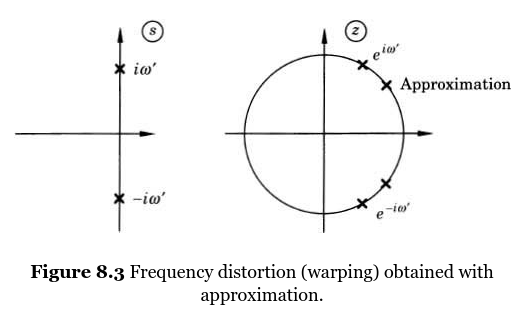
\includegraphics[width=0.6\linewidth]{../../figures/fig8_3.png}
\end{center}
The infinite positive imaginary axis in the s-plane is mapped to the finite-length upper half of the unit circle in the z-plane.
\end{frame}
\begin{frame}[label={sec:orge1d3f82}]{Exercise}
Find the discrete approximation of the lead-compensator \(F(s) = \frac{s+b}{s+a}\), and determine the pole for 
\begin{enumerate}
\item Forward difference. Substitute 
\[ F_d(z) = F(s')|_{s'=\frac{z-1}{h}}. \]
\item Backward difference. Substitute 
\[ F_d(z) = F(s')|_{s'=\frac{z-1}{zh}}. \]
\item Tustin's approximation
\[ F_d(z) = F(s')|_{s'=\frac{2}{h}\cdot \frac{z-1}{z+1}}. \]
\end{enumerate}
\end{frame}
\begin{frame}[label={sec:org5c33405}]{Forward difference exercise}
\begin{center}
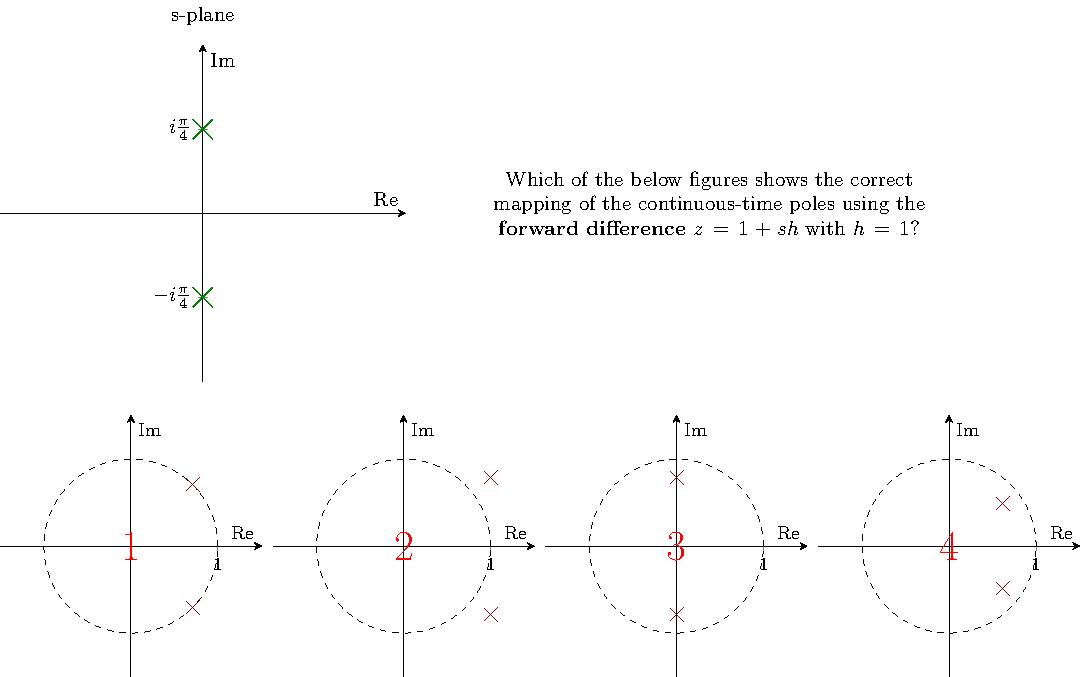
\includegraphics[width=\linewidth]{../../figures/forward-diff-exercise}
\end{center}
\end{frame}

\begin{frame}[label={sec:org357e357}]{Backward difference exercise}
\begin{center}
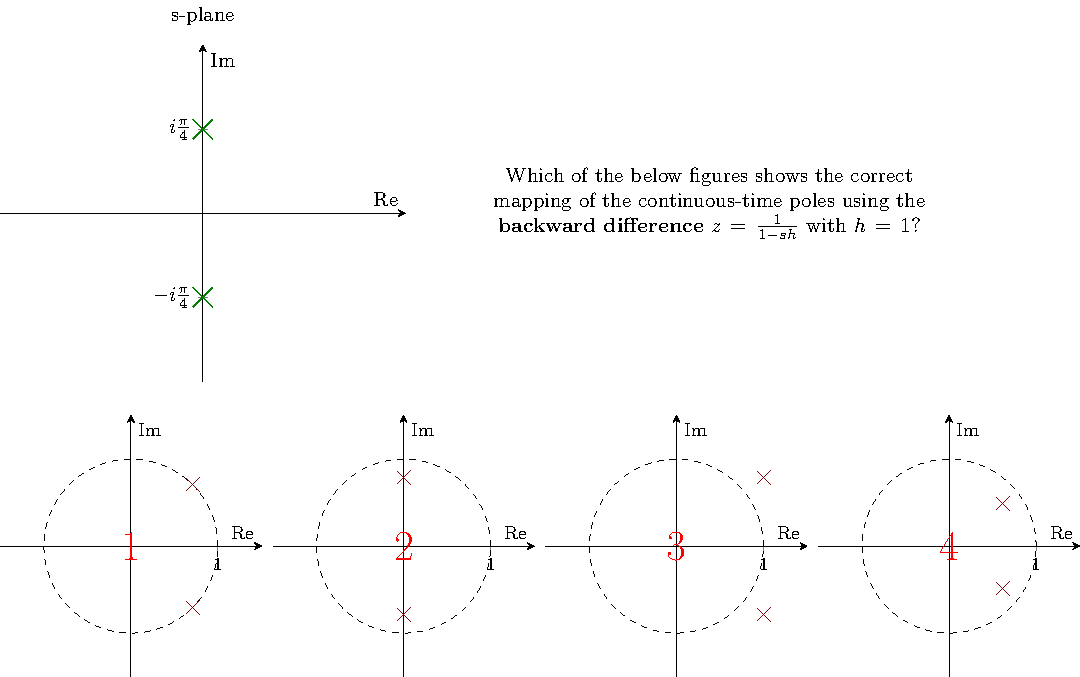
\includegraphics[width=\linewidth]{../../figures/backward-diff-exercise}
\end{center}
\end{frame}
\end{document}